%\documentclass{article}
\documentclass[a4paper,12pt]{article}
% Seitenränder in schön für Steven
%\usepackage{geometry}
%\geometry{a4paper,left=20mm,right=20mm,top=20mm,bottom=25cm}
\usepackage{enumitem}
\usepackage{amsmath}
\usepackage{graphicx}
\usepackage{tikz}
\usepackage{titling}


 

% Schusterjungen und Hurenkinder bestrafen
\clubpenalty50000
\widowpenalty50000
\displaywidowpenalty=50000

% Buchstaben mit kringel drum: %
\newcommand*\mycirc[1]{%
	\begin{tikzpicture}[baseline=(C.base)]
	\node[draw,circle,inner sep=1pt](C) {#1};
	\end{tikzpicture}}

\author{Benedikt Hans, Christoph Dollase, Steven Te\ss endorf}
\setlength{\droptitle}{-5em} % set the title to the top of the page

% ==========================
% ===== START HERE!! =======
% ==========================
\title{ \textbf{Problem Sheet 3}}
\setcounter{section}{3} % Nummer des Aufgabenblattes

\begin{document}	 
 \maketitle	 %Some Vodoo-magic
 
 \subsection{The core of the Internet}
 \paragraph{Visit the following website http://www.caida.org/research/topology/.... and have a look at the data and media they provide. Discuss the existence of an Internet core}
 \paragraph{answer:}
 % Solution
 
 coming soon$^{_{TM}}$
 
 \subsection{Reference Models}
 \paragraph{Repeat and discuss the differences in the ISO/OSI and TCP/IP models. Take a look at the session and presentation layer functions of the ISO/OSI model. Where are they implemented in the TCP/IP model? Discuss whether this is a good design decision. }
 \paragraph{answer:}
 
 \begin{itemize}[itemsep=0pt]
 	\item  ISO/OSI has 7 layers, TCP/IP has 4 layers
 	\item  Application Layer / Transport layer are in both models
 	\begin{itemize}
 		\item  Application layer in TCP/IP implenents functions from the presentation / session layers in ISO/OSI
 	\end{itemize}
 	\item  Network layer (ISO/OSI) is called Internet layer (TCP/IP)
 	\item  Data Link layer \& Physical layer are merged in the TCP/IP model, it's called Host\item To\item Network layer
 	\item  Presentation layer / Session layer are not implemented in the TCP/IP model, they're part of the application layer
 	\item  both implementations aren't perfect
 	\item  TCP/IP came earlier, ISO/OSI was rushed
 	\item  with 7 layers, ISO/OSI appears to be far more complex to implement thant TCP/IP
 	\item  partly unnecessary features in the ISO/OSI specification, thousands of pages of specification descriptions
 	\item  ISO/OSI considers too many special cases, which led to the inclusion of too many options, making the products lavish, unhandy and far too expensive
 \end{itemize}
  \begin{figure}[h!]
 	\begin{center}
 		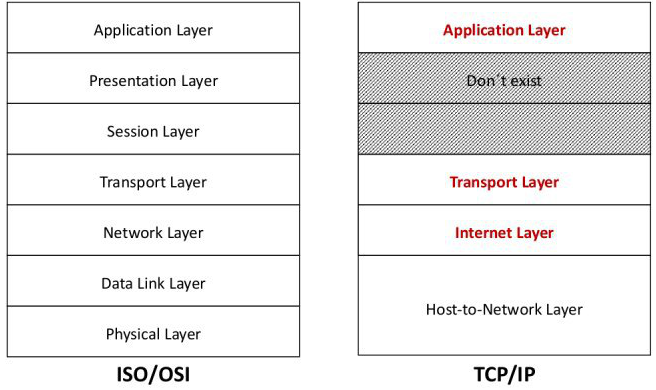
\includegraphics[width=0.7\linewidth]{TCP-OSI.png} 
 		\caption{Comparison: ISO/OSI vs TCP/IP}
 	\end{center}
 \end{figure}
 
 \subsection{Terminology}
 \paragraph{Explain what the terms throughput, goodput and packet delivery ratio describe in the context of computer networks.}
 \paragraph{answer:}
 
 \textbf{Throughput:} = Network throughput \\
 \begin{itemize}[itemsep=0pt]
 	\item  rate at which information is sent through the network
 	\item  usually measured in bits per second, sometimes in data packets per second
 	\item  also called bandwidth, data rate
 \end{itemize}

 \textbf{Goodput:}  = Application - Level throughput
 \begin{itemize}[itemsep=0pt]
 	 \item  number of useful information bits delivered by the network to a certain destination unit of time
 	\item  amount of data considered excludes protocol overhead bits and retransmitted data packets
 	\item  always lower as throughput
 \end{itemize}

 \textbf{Packet Delivery Ratio:}
 \begin{itemize}[itemsep=0pt]
 	\item  ratio of packets successfully received to the total sent
 	\item  goes hand in hand with throughput
 \end{itemize}
  
 
  \subsection{Latency and bandwith}
 \paragraph{The terms latency and bandwith have been introduced in the lecture. Discuss in which of the following application scenarios latency, bandwidth or both are most important.}
 \paragraph{answer:}

 
 \begin{enumerate}[itemsep=0pt]
	 \item FTP (file transfer)
	  \begin{itemize}[itemsep=0pt]
	 	\item bandwidth
	  \end{itemize} 
	 \item SSH (shell access)
		\begin{itemize}[itemsep=0pt]
		 	\item both are not really important
	 	\end{itemize}  
	 \item Pay-TV video streaming
	 \begin{itemize}[itemsep=0pt]
	 	\item bandwith is very important, especially with HD streams
	 \end{itemize}  
	 \item Remote controlled emergency shut\item off system
	 \begin{itemize}[itemsep=0pt]
	 	\item having a low latency and a high bandwith is nice to have
	 \end{itemize}
	 \item Telemedicine in the surgery
	 \begin{itemize}[itemsep=0pt]
	 	\item low latency (should be near zero) is very important
	 \end{itemize}
	 \item Acces to the world wide web
	 \begin{itemize}[itemsep=0pt]
	 	\item bandwidth is important for a faster access to the internet, but it doesn't really matter for a private user if it's a little slower
	 \end{itemize}
	 \item E-Mail
	 \begin{itemize}[itemsep=0pt]
	 	\item both are relatively important
	 	\item "survives" with a high latency / low bandwidth, e-mails just might take a while to be sent
	 \end{itemize}
 \end{enumerate}

 \subsection{Protocol Stack}
 \paragraph{Recapitulate the notion of vertical and horizontal communication in the context of a protocol stack.}
 \paragraph{answer:}
 
  \textbf{Vertical Communication (Adjacent Layer)}
 \begin{itemize}[itemsep=0pt]
 	\item  is done up and down the protocol stack every time anything is sent across the network and whenever anything is received
 	\item  higher levels are implemented as logical functions (in software, there is no actual physical connection)
 	\item  higher layers package data and send it down to the lower layers \\
 	$\rightarrow$ preparation for the data to be sent across the network \\
 	$\rightarrow$ data gets sent on the lowest level
 	\item  reversed process on the receiving end
 \end{itemize}
 
 
 \textbf{Horizontal Communication (Corresponding Layer)}
 \begin{itemize}[itemsep=0pt]
 	\item  each layer has its particular role \item  a set of general tasks for which it is responsible
 	\item  all layers, except for the physical layer, are only programs or algorithms running on devices
 	\item  software runnning at various layers communicates logically
 	\item  a software running at layer 5 on one machine can accomplish logical communication with a similar process running at layer 5 on another machine
 	\item  data has to be "passed down" to layer 1 on the sending machine
 	\item  data is transmitted over the physical connection to layer 1 on the other machine
 	\item  data will be forwarded upward the protocol stack of the receiving machine to layer 5 \\
 	$\rightarrow$ logical link at layer 5 without having a physical connection at that layer
 	\item  all horizontal communication requires vertical communication
 	\item  down the stack on one machine, back up the stack on the other machine
 	\item  doesn't always go down from the very top / go all the way up
 \end{itemize}
 
 \begin{figure}[h!] 
 	\begin{center}
 		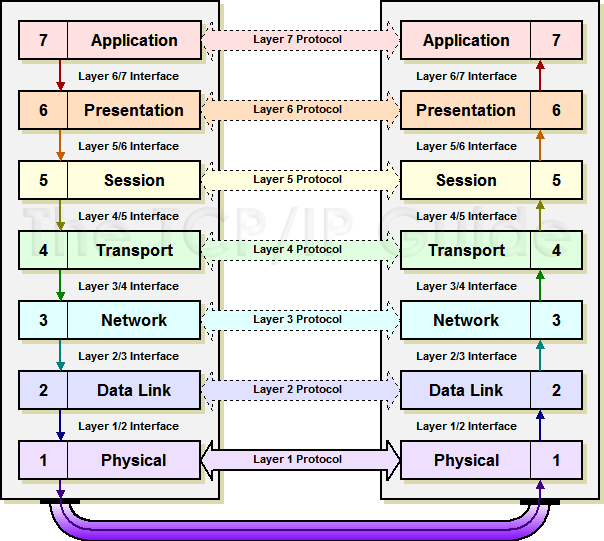
\includegraphics[width=0.8\linewidth]{OSIprotocols.png} 
 		\caption{OSI protocol layer, from: www.tcpipguide.com/free/diagrams}
 	\end{center}	
 \end{figure}
 
\end{document}

% Hier nach passiert nichts mehr, daher nutzen wir das als kleines Cheat-Sheet ;)
% ===============================================================================

% Aufzählungen (auch merhstufig):
\begin{itemize}
	\item 
\end{itemize}

%Bilder eifnügen:
\begin{figure}[h!] %h! sorgt dafür dass das Bild möglichst nicht woanders hingeschoben wird
	%Erklärung: [width=0.5\linewidth] -> Bild ist maximal so breit wie die Hälfte des Schriftbildes
	\includegraphics[width=0.5\linewidth]{Bildname.jpg} 
	\caption{Bildunterschrift}
\end{figure}

%Tabelle einfügen:
\begin{table}[h!] %h! sorgt dafür dass die Tabelle möglichst nicht woanders hingeschoben wird
	\caption{Tabellenüberschrift}
	%hinter {tabular}: Anzahl Spalten (c=center, l=linksbündig, r=rechtsbündig, | Spaltenstriche)
	\begin{tabular}{|c|c|c} 
		A & B & C  \\ % \\ = return (neue zeile)
		\hline % horinzontale Linie
		0 & 1 & 2
	\end{tabular}
\end{table}
